\label{sec:peak_detection}
In this section a tone locating algorithm will be implemented as tone location by Peak amplitude detection.
This is further tested with the specifications given in section \ref{sec:testspec}
%The integration is validated according to the test specifications in \ref{ch3}
\subsection{Note location}
To figure out which stand alone tone is being played in a given song/audio fill, to a given time, the STFT is analyzed, and the peak amplitude of the given time is located.\\
The frequency with the highest amplitude, and henceforth the largest amount of energy, is the most represented frequency. 
In an audio file, this will be the frequency of the tone being played or one of the overtones of this frequency, cf. chapter \ref{ch2}.
This will hold as long as the signal to noise ratio of the signal is not smaller than a given lower limit which is further explored in chapter \ref{ch11}.
\\
\\
A visualization of this, is finding the peaks in the output spectrogram.
Due to Heisenbergs inequality, definition \ref{theo:Heisenberg}, a compromise between the time and frequency resolution has to be made and an approximation of the notes being played is a possibility.
For a final detection, the calculated frequency would need to be compared with the frequency of the tones a guitar would play. 
This will make an approximation of the note a possibility even with a lower resolution in frequency.
\\
With the signal short time Fourier transformed, each segmented data set corresponding to a FFT of a given time, and hence finding the peak amplitude and the corresponding frequency gives the tone being played at a given time.
\\\\
To make sure that the amplitude is from a note being played, and not from noise in the signal, a check can be implemented in the algorithm, such that the amplitude is set to $0$ if the amplitude is not larger than a given limit.
This i turn will reduce the amount of noise slipping through the algorithm for signals with a low $SNR$

An algorithm for locating the frequency with the largest amplitude is implemented in python 
\begin{algorithm}[H]
\caption{Amplitude peak detection of short time Fourier transfrom}
\label{alg:FIR}
\begin{algorithmic}[1] 
\Procedure{Compute peak amplitude}{}
\State  $X$ = STFT(signal) \Comment {Given STFT calculation in an array $X$}
\State $Y =$ linspace($0,$ Nyquist, length W) \Comment Generate linear spaced vectors with len($W$) points.
	\For {each integer $i$ in length of $X$}
		\State $A = max(X[i])$ \Comment {Maximum amplitude for each FFT}
		\If {$A >$ limit} \Comment {Check if the amplitude is larger than a given limit}
			\State freq\_pos[i] = where in $X$[i], $(A == max(X[i]))$ \Comment {The location of the max amplitude is located}
		\Else
			\State freq\_pos[i] = 0	\Comment {Returns $0$ for every frequency under given amplitude}
		\EndIf
		\If {freq[i] == 0}
			\State max\_freq\_time = 0
		\Else
			\State max\_freq\_time = $Y$[freq\_pos]
		\EndIf
	\EndFor
	\State Return max\_freq\_time
\EndProcedure
\end{algorithmic}
\end{algorithm}

%An argument coud be made for looking at the 3+ higest frequencies in the signal.
\subsection{Validation of peak detection algorithm}
The algorithm is tested as stated by the specifications section \ref{sec:testspec} by feeding a STFT of a noise filled audio file containing an "$E_2$" tone being played on a guitar. 
The expected result of this test is either the fundamental of the $E_2$ = $82.41$ Hz. or an overtone of this as explained in \ref{ch2} exampled given: $\{82.41 \cdot 2 = 164.82, 82.41 \cdot 3 = 247.23, \dots \}$ 

\begin{figure}[H]
\centering 
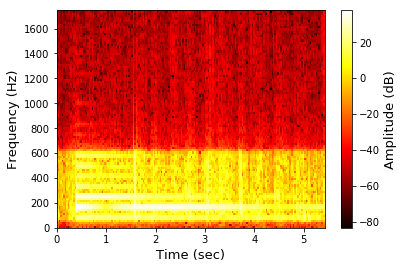
\includegraphics[width=0.5\textwidth]{figures/peak_detection/20170511_spectogram_E_2.png}
\label{fig:spec_E_2}
\caption{Spectrogram of E$_2$}
\end{figure}


\begin{figure}[H]
\centering
\begin{subfigure}{0.49\textwidth}
\centering
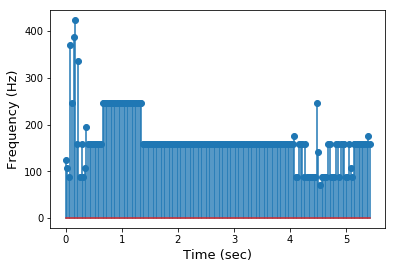
\includegraphics[width=\textwidth]{figures/peak_detection/20170511_-3.png}
\caption{Peak amplitude plotted with minimum amplitude representation of -3dB}
\label{fig:freq_-3dB_Amp_pass}

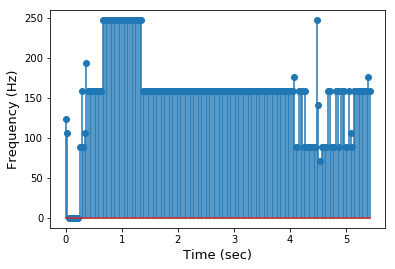
\includegraphics[width=\textwidth]{figures/peak_detection/20170511_10.png}
\caption{Peak amplitude plotted with minimum amplitude representation of 10dB}
\label{fig:freq_10dB_Amp_pass}

\end{subfigure}
\begin{subfigure}{0.49\textwidth}
\centering
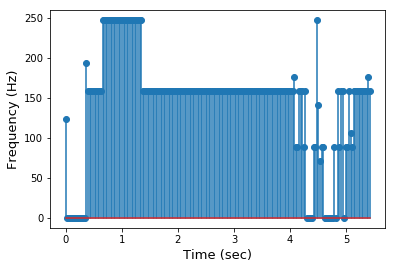
\includegraphics[width=\textwidth]{figures/peak_detection/20170511_15.png}
\caption{Peak amplitude plotted with minimum amplitude representation of 15dB}
\label{fig:freq_15dB_Amp_pass}

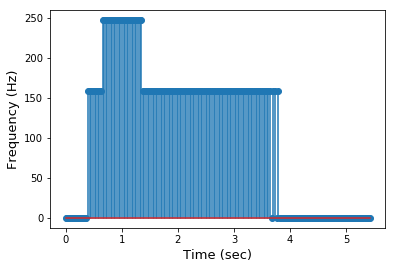
\includegraphics[width=\textwidth]{figures/peak_detection/20170511_25.png}
\caption{Peak amplitude plotted with minimum amplitude representation of 25dB}
\label{fig:freq_25dB_Amp_pass}

\end{subfigure}
\caption{Peak detection of spectrogram of $E_2$ with different amplitude limits}
\label{fig:valdation_peak_detection}
\end{figure}

The most represented frequencies in \ref{fig:spec_E_2} are $158.76$ Hz, followed by $246.96$ Hz and $88.2$ Hz. 
Knowing that the tone being played is E$_2$ with the previously mentioned fundamental and overtones, an error margin on around $6$ Hz between the expected output and the out put can be seen.
This can be due to either the guitar not playing a clean E$_2$ or previously mentioned lack of resolution in frequency.
%But can be deemed withen the limit of of approximation of a tone.

On \ref{fig:valdation_peak_detection} the effect of the chosen cut off check, can be seen.
With a low enough magnitude limit, as seen in \ref{fig:freq_-3dB_Amp_pass} none of the maximum amplitudes are removed.
This in turn makes any noise in the system able to be represented as a peak, when nothing is being played by the guitar.
Figure \ref{fig:freq_25dB_Amp_pass} is more akin to, an expected result with only overtones of the E$_2$.
If the limit is large enough, the tone being played is cut short when the amplitude of the tone descends as the tone lingers.
A compromise between letting noise pass the peak detection and cutting the note short, can be made to make sure the correct frequencies is located and the length of the tone is maintained.